\documentclass{article}
\usepackage{graphicx}
\usepackage[dvipsnames,table]{xcolor}
\usepackage[utf8]{inputenc}
\usepackage{siunitx}
\usepackage[american,siunitx]{circuitikz}
\usepackage{amsmath}
\usepackage{svg}
\usepackage{booktabs}
\usepackage{float}
\usepackage{xparse, xfp}
\usepackage{multirow}
\usepackage{tikz}
\usepackage{karnaugh-map}
\usepackage{pdfpages}
\usepackage{hyperref}
\usepackage{adjustbox}

\hypersetup{
    colorlinks=true,
    linkcolor=blue,
    filecolor=magenta,      
    urlcolor=cyan,
}
\usetikzlibrary{calc}
%\usepackage[landscape]{geometry}
\renewcommand{\thesubsection}{\thesection.\alph{subsection}}
\newcommand{\equal}{=}
\newcommand{\greyrule}{\arrayrulecolor{black!30}\midrule\arrayrulecolor{black}}
\makeatletter
\newcommand\currcoor{\the\tikz@lastxsaved,\the\tikz@lastysaved}
\makeatother
\newcolumntype{:}{@{\hskip\tabcolsep\color{black!30}\vrule\hskip\tabcolsep}}

\ExplSyntaxOn
\NewExpandableDocumentCommand \groupify { O{\,\allowbreak} m m }
  { \jakob_groupify:nnn {#1} {#2} {#3} }
\cs_new:Npn \jakob_groupify:nnn #1 #2 #3
  { \__jakob_groupify_loop:nnw { 1 } {#2} #3 \q_recursion_tail {#1} \q_recursion_stop }
\cs_new:Npn \__jakob_groupify_loop:nnw #1 #2 #3
  {
    \quark_if_recursion_tail_stop:n {#3}
    \exp_not:n {#3}
    \int_compare:nNnTF {#1} = {#2}
      { \__jakob_groupify_sep:n }
      { \exp_args:Nf \__jakob_groupify_loop:nnw { \int_eval:n { #1+1 } } }
          {#2}
  }
\cs_new:Npn \__jakob_groupify_sep:n #1 #2 \q_recursion_tail #3
  {
    \tl_if_empty:nF {#2} { \exp_not:n {#3} }
    \__jakob_groupify_loop:nnw { 1 } {#1}
    #2 \q_recursion_tail {#3}
  }
\ExplSyntaxOff

\title{ECE 2200L\\Introduction to Microelectronics Circuits Laboratory\\\,\\Experiment 3\\Applications of the PN Diode\\\,\\Report}
\author{Choi Tim Antony Yung}
\date{September 23, 2020}
\begin{document}
\maketitle

\thispagestyle{empty}
\setcounter{page}{0}

\newpage

\section*{Objective}

To experiment on some examples of the applications of PN diodes as non-linear circuit elements. Specifically, rectifiers, peak detectors as DC power supplies, and clippers/limiters will be studied.
\section*{Result}

\subsection*{Circuit 1}

\begin{figure}[H]
  \centering
  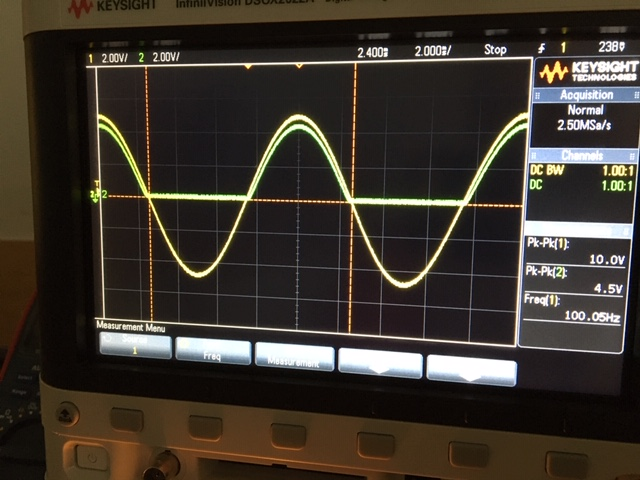
\includegraphics[width=\textwidth]{image/Part1/IMG_3693.JPG}
  \caption{Oscilloscope plot demonstrating input and output voltage with $V_{in}=5\text{V}_{pk}$}
\end{figure}
\begin{figure}[H]
  \centering
  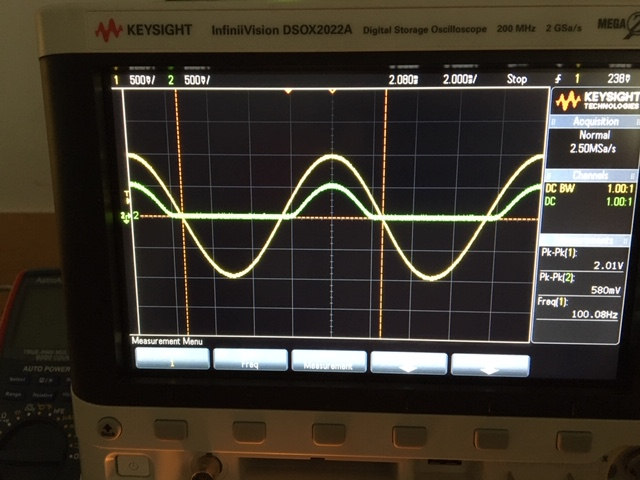
\includegraphics[width=\textwidth]{image/Part1/IMG_3694.JPG}
  \caption{Oscilloscope plot demonstrating input and output voltage with $V_{in}=1\text{V}_{pk}$}
\end{figure}\begin{figure}[H]
  \centering
  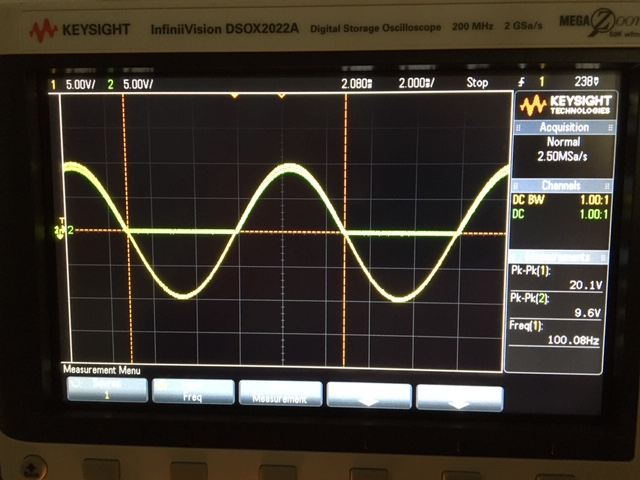
\includegraphics[width=\textwidth]{image/Part1/IMG_3696.JPG}
  \caption{Oscilloscope plot demonstrating input and output voltage with $V_{in}=10\text{V}_{pk}$}
\end{figure}

\begin{table}[H]
  \centering
    \begin{tabular}{rr}
      \toprule
    \multicolumn{1}{l}{$Vin_{pk}$ (V)} & \multicolumn{1}{l}{$Vout_{pk}$ (V)} \\
    \midrule
    1     & 0.58 \\
    5     & 4.5 \\
    10    & 9.6 \\
      \bottomrule
  \end{tabular}%
    \caption{Peak value of output voltage as input voltage changes}
\end{table}%

\begin{figure}[H]
  \centering
  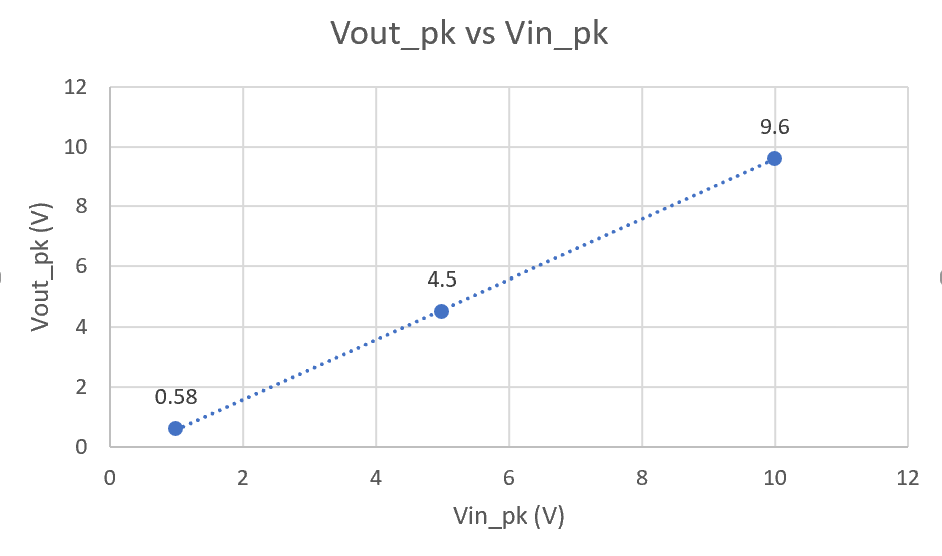
\includegraphics[width=\textwidth]{image/Part1/plot.png}
  \caption{$Vout_{pk}$ vs. $Vin_{pk}$ plot}
\end{figure}

\subsection*{Circuit 2}

\begin{figure}[H]
  \centering
  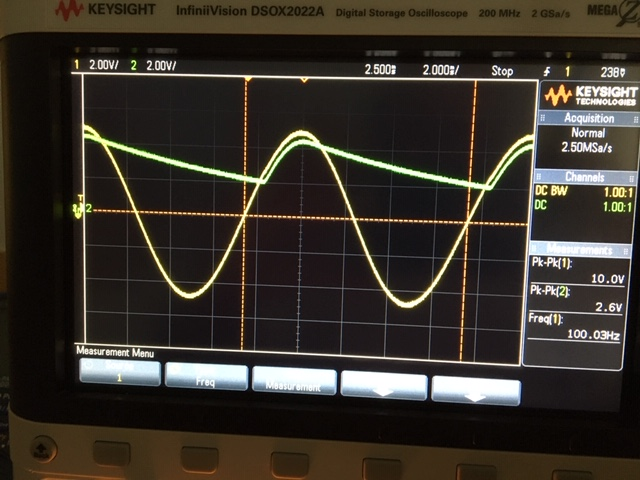
\includegraphics[width=\textwidth]{image/Part2/1u10k.JPG}
  \caption{Oscilloscope plot demonstrating input and output voltage with \SI{1}{\micro\farad} capacitor and \SI{10}{\kilo\ohm} resistor}
\end{figure}
\begin{figure}[H]
  \centering
  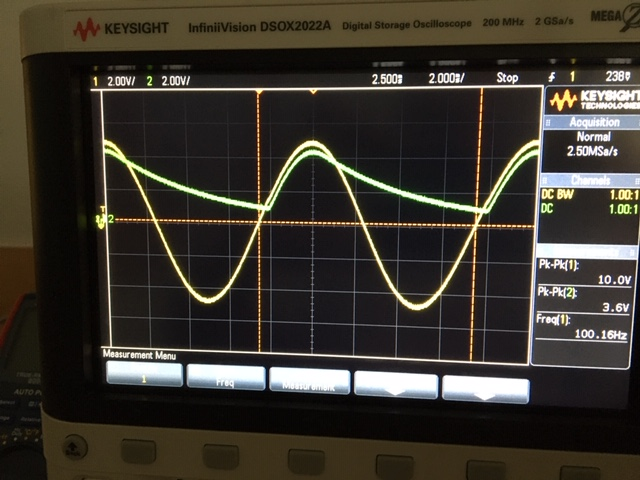
\includegraphics[width=\textwidth]{image/Part2/1u4k7.JPG}
  \caption{Oscilloscope plot demonstrating input and output voltage with \SI{1}{\micro\farad} capacitor and \SI{4.7}{\kilo\ohm} resistor}
\end{figure}
\begin{figure}[H]
  \centering
  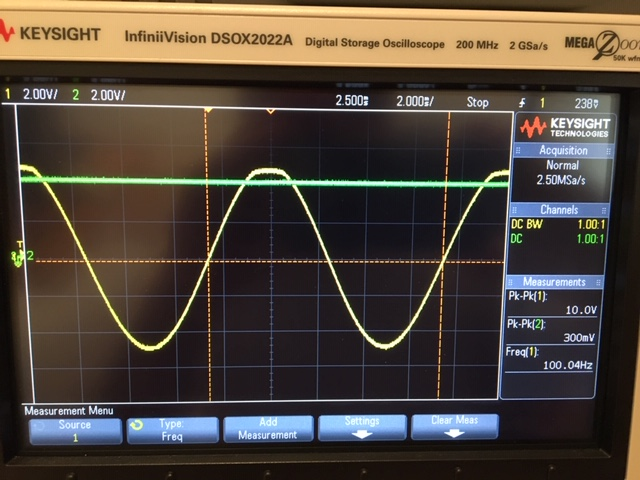
\includegraphics[width=\textwidth]{image/Part2/100u10k.JPG}
  \caption{Oscilloscope plot demonstrating input and output voltage with \SI{100}{\micro\farad} capacitor and \SI{10}{\kilo\ohm} resistor}
\end{figure}

\begin{table}[H]
  \centering
    \begin{tabular}{rrr}
      \toprule
      \multicolumn{1}{l}{f (Hz)} & \multicolumn{1}{l}{$\frac{1}{f}$ (s)} & \multicolumn{1}{l}{$Vr_{pp}$ (V)} \\
      \midrule
      50    & 0.02  & 3.7 \\
      100   & 0.01  & 2.7 \\
      200   & 0.005 & 1.7 \\
      400   & 0.0025 & 1 \\
      600   & 0.001667 & 0.8 \\
      800   & 0.00125 & 0.56 \\
      1000  & 0.001 & 0.44 \\
      \bottomrule
  \end{tabular}%
    \caption{Peak-to-peak value of output voltage as frequency changes}
\end{table}%

\begin{figure}[H]
  \centering
  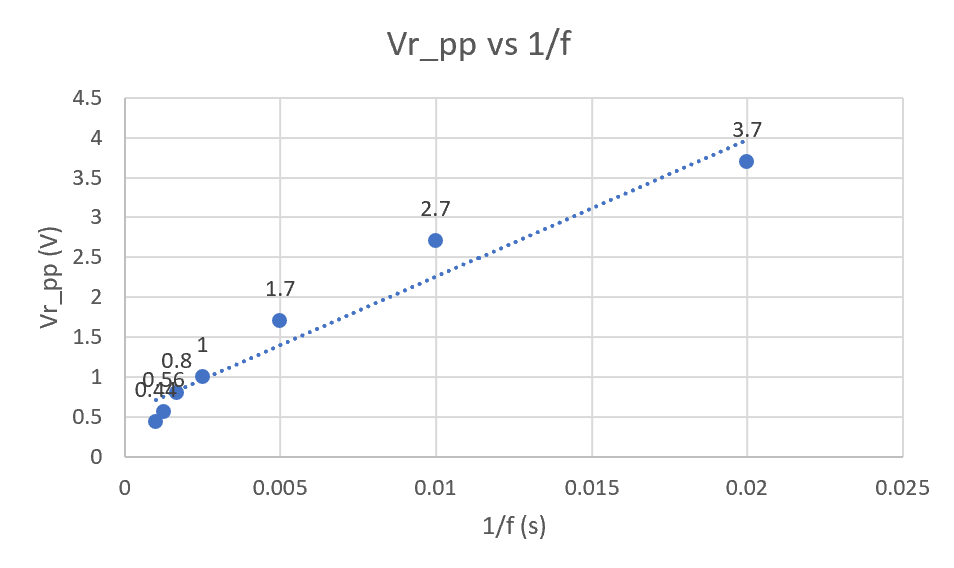
\includegraphics[width=\textwidth]{image/Part2/plot.png}
  \caption{$Vout_{pp}$ vs. $\frac{1}{f}$ plot}
\end{figure}

\newpage

\subsection*{Circuit 3}

According to \href{https://www.onsemi.com/pub/Collateral/1N4001-D.PDF}{1N4001 datasheet from ON Semiconductor}, the average forward voltage drop of 1N4001 is \SI{0.8}{\volt}. Therefore, as $V_{in}$ increases pass \SI{5.8}{\volt}, $V_{out}$ will be limited by the middle branch of the circuit to \SI{5.8}{\volt}. As $V_{in}$ decreases pass \SI{-5.8}{\volt}, $V_{out}$ will be limited by the right branch of the circuit to \SI{-5.8}{\volt}.
\begin{figure}[H]
  \centering
  \begin{adjustbox}{max width=\textwidth}
\begin{tikzpicture}
  \draw
  (-10,0) -- (10,0) node[right]{$V_{in}$}
  (0,-10) -- (0,10) node[above]{$V_{out}$}
  (5.8,0.25) -- (5.8,-0.25) node[below]{5.8}
  (-5.8,0.25) -- (-5.8,-0.25) node[below]{-5.8}
  (0.25,5.8) -- (-0.25,5.8) node[left]{5.8}
  (0.25,-5.8) -- (-0.25,-5.8) node[left]{-5.8}
  ;
  
  \draw [line width=0.5mm, black]
  (-10,-5.8) -- (-5.8,-5.8)
  (-5.8,-5.8) -- (5.8,5.8)
  (5.8,5.8) -- (10,5.8)
  ;
\end{tikzpicture}
\end{adjustbox}
\caption{$V_{out}$ vs $V_{in}$ plot in theory with 1N4001 forward voltage drop as \SI{0.8}{\volt}}
\end{figure}

\begin{figure}[H]
  \centering
  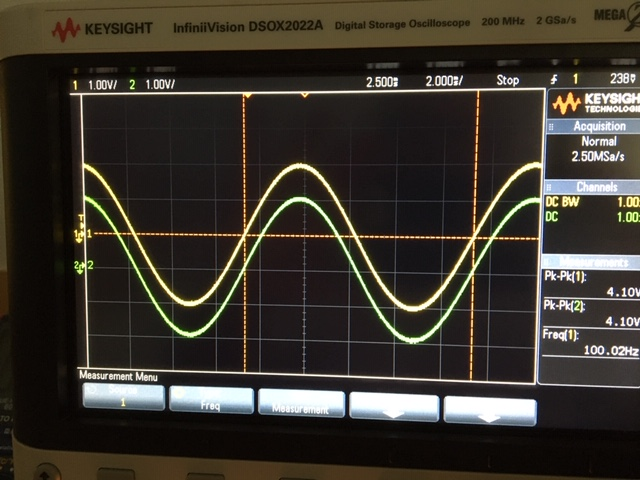
\includegraphics[width=\textwidth]{image/Part3/IMG_3701.JPG}
  \caption{Oscilloscope plot demonstrating input and output voltage with $V_{in}=2\text{V}_{pk}$}
\end{figure}
\begin{figure}[H]
  \centering
  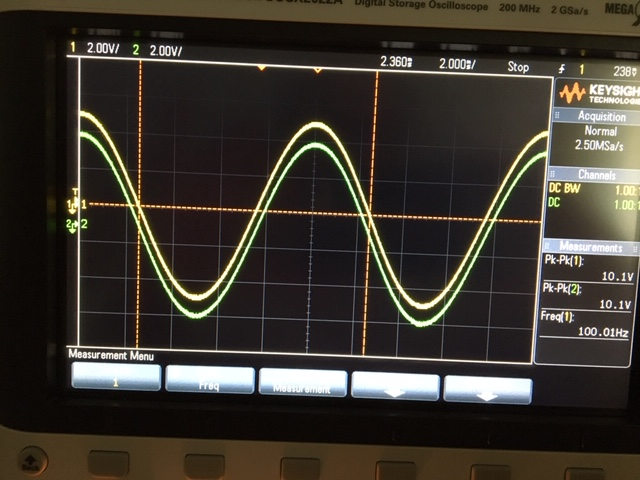
\includegraphics[width=\textwidth]{image/Part3/IMG_3702.JPG}
  \caption{Oscilloscope plot demonstrating input and output voltage with $V_{in}=5\text{V}_{pk}$}
\end{figure}
\begin{figure}[H]
  \centering
  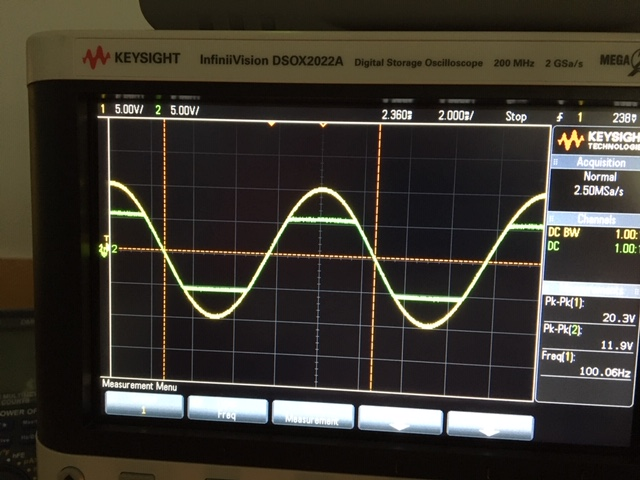
\includegraphics[width=\textwidth]{image/Part3/IMG_3703.JPG}
  \caption{Oscilloscope plot demonstrating input and output voltage with $V_{in}=10\text{V}_{pk}$}
\end{figure}
\begin{figure}[H]
  \centering
  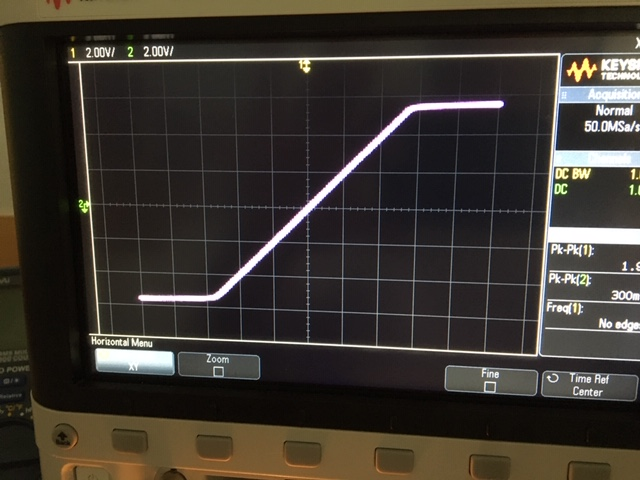
\includegraphics[width=\textwidth]{image/Part3/IMG_3704.JPG}
  \caption{Oscilloscope plot of $V_{out}$ vs $V_{in}$}
\end{figure}

\begin{table}[H]
  \centering
    \begin{tabular}{rr}
      \toprule
    \multicolumn{1}{l}{$Vin_{pk}$ (V)} & \multicolumn{1}{l}{$Vout_{pk}$ (V)} \\
    \midrule
    1     & 0.58 \\
    5     & 4.5 \\
    10    & 9.6 \\
      \bottomrule
  \end{tabular}%
    \caption{Peak value of output voltage as input voltage changes}
\end{table}%

As can be seen from the Oscilloscope plot similar to the theoretical plot, the circuit behaved as expected.

\section*{Conclusion}
Various application of diode, specifically half-wave rectifier, peak detector and clipper circuit. As can be seen form the result, the diode have an effect of a small decrease in peak load voltage in a helf-wave rectifier circuit; the configuration of larger resistance and capacitance have an effect of decreasing the magnitude of ripple on the output voltage; and the clipper circuit characteristics is observed.


\end{document}
